
%(BEGIN_QUESTION)
% Copyright 2011, Tony R. Kuphaldt, released under the Creative Commons Attribution License (v 1.0)
% This means you may do almost anything with this work of mine, so long as you give me proper credit

Calculate the straight-line distances between the following {\sl Wireless}HART instruments, based on locations shown on this plot plan of an industrial processing unit.  Each division on the map is equivalent to a distance of 5 feet:

$$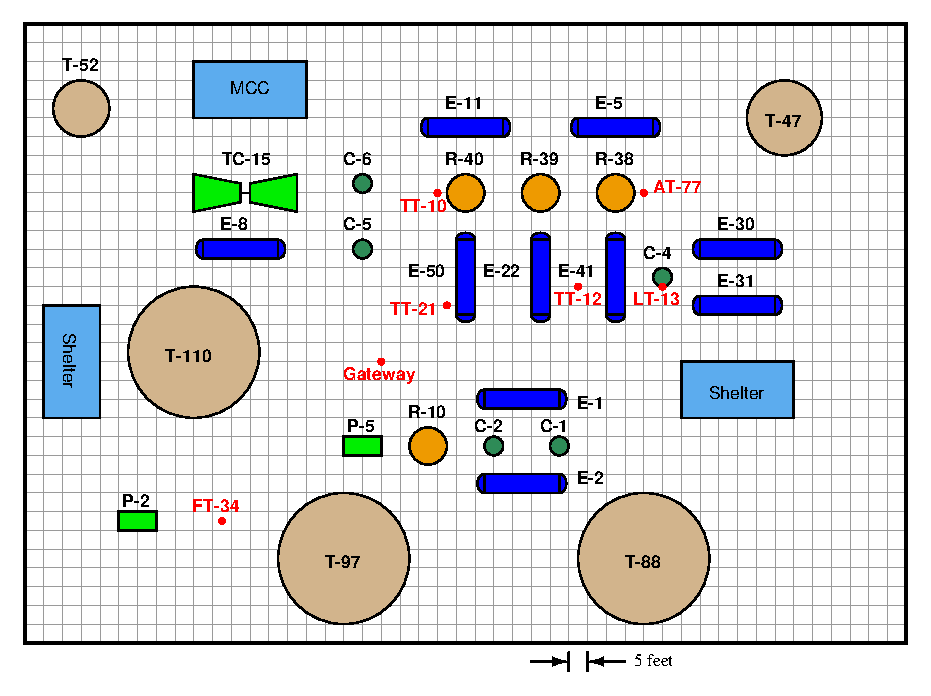
\includegraphics[width=15.5cm]{i03476x01.eps}$$

\begin{itemize}
\item{} Distance from Gateway to TT-10 = \underbar{\hskip 50pt} 
\vskip 10pt
\item{} Distance from TT-21 to FT-34 = \underbar{\hskip 50pt} 
\end{itemize}

\underbar{file i03476}
%(END_QUESTION)





%(BEGIN_ANSWER)

\begin{itemize}
\item{} Distance from Gateway to TT-10 = {\bf 47.434 feet} 
\item{} Distance from TT-21 to FT-34 = {\bf 83.104 feet} 
\end{itemize}

%(END_ANSWER)





%(BEGIN_NOTES)

{\bf This question is intended for exams only and not worksheets!}

%(END_NOTES)


